\chapter{Background}
\label{cha:background}

This chapter gives the background information required to understand the rest of
this report. If the reader is already well-versed in Spoofax and familiar with
the concept of a REPL, this chapter can be skipped.

The first section, \cref{sec:spoofax}, briefly explains what Spoofax is and what
services it provides to the language designer. \Cref{sec:repl} gives a quick
overview of what a REPL is and what advantages it offers to programmers.

\section{The Spoofax Language Workbench}
\label{sec:spoofax}
Spoofax is a platform that allows for giving a completely \emph{declarative}
definition of a programming language and accompanying integrated development
environment (IDE) support~\cite{Kats10a}. Such a platform is called a
\emph{language workbench}.

In discussing programming languages, it is useful to distinguish the following
three concepts: an \textit{aspect} of a language, the formal
\textit{specification} of that aspect, and the actual \textit{implementation} of
that aspect that adheres to the specification. Any programming language can be
divided into multiple distinct aspects. In \cref{fig:spoofax-relations}, four
common aspects of programming languages are shown, along with the relation
between the formal specification and implementation for each aspect. An example
of an aspect is the \textit{syntax}: its formal specification is done with
grammar rules, and its implementation traditionally consists of both a tokenizer
and parser.

A key property of Spoofax is that it allows a language designer to give a
complete specification of each aspect of their language, and automatically
derives the implementations of those aspects from their respective
specifications. Spoofax provides a range of high-level, declarative
\textit{meta-languages} to declare language specifications.

This section goes over the aspects that come into play with the development of a
language and how Spoofax tackles each of these aspects with its
meta-languages. First, the section goes over some of the elements that make up
the specification of each language aspect\footnote{This section follows the
  structure of the language specification portion of the compiler construction
  course at the TU Delft. The slides can be found here:
  \url{http://tudelft-in4303.github.io/lectures/specification/}.}. A language
commonly consists of the following aspects, shown also in
\cref{fig:spoofax-relations}, of which a selection is discussed in more
detail throughout the rest of this section:

\begin{enumerate}
\item \textbf{\hyperref[ssec:syntax-def]{Syntax}:} The first aspect concerns
  what textual representations of a program are syntactically valid. Its
  specification consists of a grammar specified with context-free grammar
  productions. A parser provides an implementation of this specification, by
  mapping a textual representation of a program to an abstract syntax tree (AST)
  representation. In Spoofax, the syntax is declared with a domain specific
  language (DSL) called SDF3.
\item \textbf{Static semantics:} A parsed AST then optionally goes through
  static analysis (type checking, name binding and variable scoping), to test if
  the program is well-formed. Static analysis is the implementation of an aspect
  called \textit{static semantics}. The static semantics of a language can be
  formally specified by \textit{type and/or name binding rules}. Spoofax
  provides two DSLs that can specify the two distinct parts of the
  specification: the TS Type Specification language and the NaBL name binding
  language.

  This language aspect is not discussed in this section, but it is explained in
  the research report in \cref{ssec:a-static-analysis}.
\item \textbf{Term rewriting or program transformation:} A well-formed AST can
  then be transformed, for example for desugaring or optimization. This
  execution step falls under the aspect of \textit{term rewriting} and can be
  formally specified by \textit{term rewrite rules}. For the specification of
  this aspect, Spoofax provides a DSL called Stratego.

  This aspect is also not discussed in this section, the relevant section from
  the research report can be found in \cref{ssec:a-term-rewrite}.
\item \textbf{\hyperref[ssec:dynamic-semantics]{Dynamic semantics}:} Next the
  transformed AST is either compiled or interpreted, thereby providing a means
  of execution. The aspect of \textit{dynamic semantics} defines what the
  behavior is of a program upon execution. The formal specification of this
  aspect can be done with \textit{reduction rules}, although there are other
  ways to accomplish this. For example, interpretation can be seen as the
  transformation of a program to a single value. In Spoofax, the dynamic
  semantics can be defined with either Stratego or a DSL called DynSem.
\end{enumerate}

\begin{figure}[t]
  \centering
  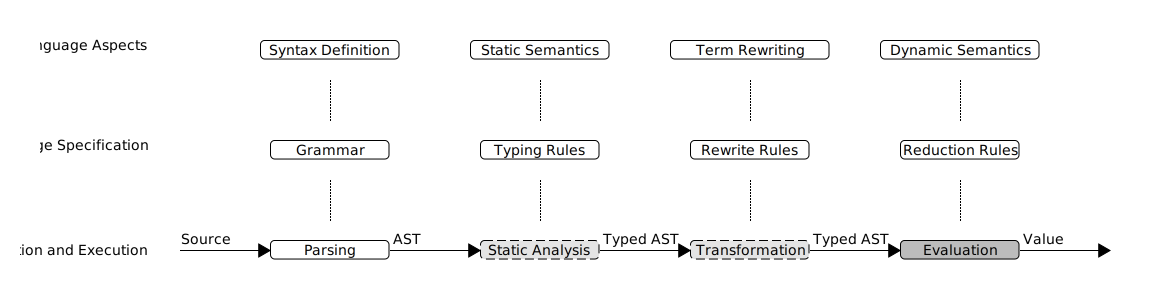
\includegraphics[width=\textwidth]{spoofax-relations}
  \caption{The relations between the aspects of a programming language, their
    specifications and their implementations. The dashed boxes in the bottom row
    indicate optional steps.}
  \label{fig:spoofax-relations}
\end{figure}

After the explanation of the language aspects, this section concludes with a
discussion on the other part of a language: its IDE. Spoofax provides IDE
support by means of its \textit{editor services}.

\subsection{Syntax}
\label{ssec:syntax-def}
The first part of the specification of a language is its syntax. The
syntax of a language is often specified by means of a \emph{lexical
grammar} and a \emph{context-free grammar}, as can be seen in the
specification of, for example, Standard ML~\cite{Milner97}. The
lexical grammar is most often defined using regular expressions. It
defines the individual words made up of characters, such as
identifiers and numeric constants. The context-free grammar then
defines syntactically valid sentences made up of words.

\subsubsection{SDF3: syntax definition in Spoofax}
\label{ssec:orgheadline1}
To specify a syntax definition declaratively in Spoofax, a DSL called
SDF3~\cite{Vollebregt12} is used.  SDF3 is the third generation
of the \emph{Syntax Definition Formalism} (SDF)~\cite{Heering89}. It
uses only context-free grammar productions for the specification of
both the lexical syntax and the context-free syntax, a feature that
was introduced in SDF2~\cite{Visser97}.

The declarative nature of SDF3 allows for thinking in terms of the
structure (the \emph{what}), instead of in terms of parser algorithms (the
\emph{how}) as is the case with many current parser generators such as
ANTLR and YACC~\cite{Kats10b}. The syntax definition is used to
make parsers that parse a textual representation of a program into its
AST and pretty-printers for mapping ASTs back to text. However, due to
its declarative nature, SDF3 is not limited to generating parsers and
pretty printers: it can also be used for error recovery
rules~\cite{deJonge12}, syntax highlighting rules and folding
rules for editors (see \cref{ssec:editor-serv}).

The Spoofax API gives access to the generated parser through the
\texttt{SyntaxService}. The results obtained by executing the parser results in,
among other information, an AST represented as an internal data structure. This
data structure is briefly highlighted in the following section.

\subsubsection{ASTs in Spoofax: Stratego terms}
\label{sec:asts-spoof-strat}
In Spoofax, an AST is represented as a Stratego term~\cite{Kats10a}. Terms in
Spoofax come with a textual format called the ATerm Format~\cite{Brand00}. As an
example, a term representation of the arithmetic expression $2 + 2 - 4$ is shown
in \cref{lst:aterm-example}.

\begin{lstlisting}[caption={An example ATerm representation of an arithmetic
expression.},language=aterm,label={lst:aterm-example}]
Sub(Add(Int("2"), Int("2")), Int("4"))
\end{lstlisting}

Terms can however represent any tree structure, not just ASTs. For example, a
term may just as well represent a value. As such, when using Spoofax
programmatically through its API, one sees terms used as an internal
representation of the data going through the execution pipeline as depicted in
\cref{fig:spoofax-relations}.

\subsection{Dynamic semantics}
\label{ssec:dynamic-semantics}
Dynamic semantics refers to how a program written in some language
behaves~\cite{Winskel93}. There are many approaches to formally specify the
dynamic semantics of a programming language (for an extensive treatment, see
``\usebibentry{Winskel93}{title}''~\cite{Winskel93}). One way, for example, is
to specify the compilation to a different high-level language of which the
dynamic semantics are already known.

\subsubsection{DynSem: rule-based dynamic semantics}
\label{ssec:dynsem}
Aside from Stratego, the Spoofax team has developed an additional method to
declare the dynamic semantics of a language, namely a DSL called
DynSem~\cite{VerguNV15}. DynSem allows for an operational semantics
specification from which a Java-based AST interpreter can be automatically
derived.

DynSem uses an approach called \textit{operational semantics}. The rest of this
section discusses how DynSem (and operational semantics) is used to specify the
dynamic semantics of a language in Spoofax.

\paragraph{Reduction rules} In DynSem and operational semantics, reduction rules
are used to specify the dynamic semantics of a language. The syntax of a DynSem
specification is similar to the formal syntax as shown in
equation~(\ref{eq:formal-spec}), which will be discussed later in more
detail. \Cref{lst:dynsem-rule-syntax} shows the syntax of a reduction rule as
specified in DynSem.
% NOTE: do _not_ change the above \ref to \cref, as it will render the label as
% figure. See the hack below for more info.

\begin{minipage}[t]{\linewidth}
\begin{lstlisting}[language=dynsem,numbers=left,caption={The syntactic structure
of a reduction rule in DynSem.},label={lst:dynsem-rule-syntax}]
  Rs |- <term1> :: RWs --> <term2> :: RWs'
  where <premise1>;
        <premise2>.
\end{lstlisting}
\end{minipage}

A reduction rule consists of a set of premises (lines 2 and 3) and a conclusion
(line 1). Put simply, the conclusion of a reduction rule holds if all of its
premises hold~\cite{Kahn87}. Thus, the rule shown in
\cref{lst:dynsem-rule-syntax} is read as follows: given that the premises
\texttt{premise1} and \texttt{premise2} hold, the conclusion in line 1 holds.

The left-hand side of the conclusion, the terms to the left of the arrow,
represents a pattern match on terms, matching variables that can be referenced
in other places of the rule. The right-hand side of the conclusion represents an
instantiation of terms, and is called the result of the
reduction~\cite{VerguNV15}.

\paragraph{Semantic components} The variables \texttt{Rs}, \texttt{RWs} and
\texttt{RWs'} shown in \cref{lst:dynsem-rule-syntax} are called \textit{semantic
  components}: they represent the context in which the reduction takes place. An
example of a semantic component is that of an environment, which maps variable
names to their values. Another example is that of a store, which maps addresses
of values to the values themselves.

There are two kinds of semantic components: \textit{read-only} semantic
components and \textit{read-write} semantic components. An environment is a
read-only semantic component: a variable is bound only within a certain scope,
and any other reduction rules that are applied outside of that scope do not see
this environment. A store is a read-write semantic component: changes in the
store are visible everywhere, as it represents mutable state.

\paragraph{Specifying function application in DynSem} An example of a reduction
rule specified in DynSem is shown in \cref{lst:dynsem}. The rule specifies the
semantics of function application by using an environment. Next to it, in
equation~(\ref{eq:formal-spec}), the same rule is shown in a formal syntax, to
highlight the similarity of DynSem's syntax with that of a formal one.

\begin{minipage}[t]{\linewidth}
\begin{minipage}{0.45\textwidth}
\begin{lstlisting}[language=dynsem,numbers=left]
rules
  App(ClosV(x, e, E), v1) --> v2
  where
    E  |- bindVar(x, v1) --> E';
    E' |- e --> v2.
\end{lstlisting}
\end{minipage}
\begin{minipage}{0.55\textwidth}
  \centering
  \begin{equation*}
    \infer{%
      \left(\lambda x.e, E\right)~e_1 \longrightarrow v%
    }{%
      (x \mapsto e_1) \circ E \longrightarrow E' &\quad E' \vdash e \longrightarrow v
    }
  \end{equation*}
\end{minipage}
\\
\begin{minipage}[t]{0.47\textwidth}
  \captionof{lstlisting}{Specifying function application through the use of an
    environment.}\label{lst:dynsem}
\end{minipage}
\hspace{0.02\textwidth}
\begin{minipage}[t]{0.5\textwidth}
  % Hack: Locally change to use figure counter and label.
  \renewcommand*\figurename{Equation}
  \makeatletter
    \let\c@figure\c@equation
  \makeatother
  \captionof{figure}{The same rule in a formal specification. Here, the premises
  are shown on top.}\label{eq:formal-spec}
\end{minipage}
\end{minipage}

The rule first introduces a pattern-match on a term representing function
application on a closure (i.e. a function together with its enclosing
environment \texttt{E}). In line 4, the environment \texttt{E} (a semantic
component) is extended with a variable binding \texttt{x $\mapsto$ v1} to form a
new environment \texttt{E'}. Then, in line 5, the function body \texttt{e} is
reduced to the value \texttt{v2}, within the context of the newly extended
environment \texttt{E'}.

\subsection{Editor services}
\label{ssec:editor-serv}
This section concludes with a brief description of editor services,
which provide the IDE support for languages defined in
Spoofax. Examples of such services include an outline view, menus in
which one can bind actions to menu buttons (see
\cref{fig:menu-actions}), but also syntax highlighting, syntactic code
completion and code folding rules\footnote{More services are
listed on the Spoofax website:
\url{https://web.archive.org/http://www.metaborg.org/spoofax/editor-services/}}.

The Spoofax API provides the editor services with similar naming. For
example, the outline can be retrieved from the \texttt{OutlineService}, the
syntax highlighting can be accessed through the \texttt{StylerService} and
syntactic code completion is accessed with the
\texttt{CompletionService}. The defined menus for a particular language can
be retrieved with the \texttt{MenuService}, from which the menu actions can
be retrieved and used.

\begin{figure}[bt]
\centering
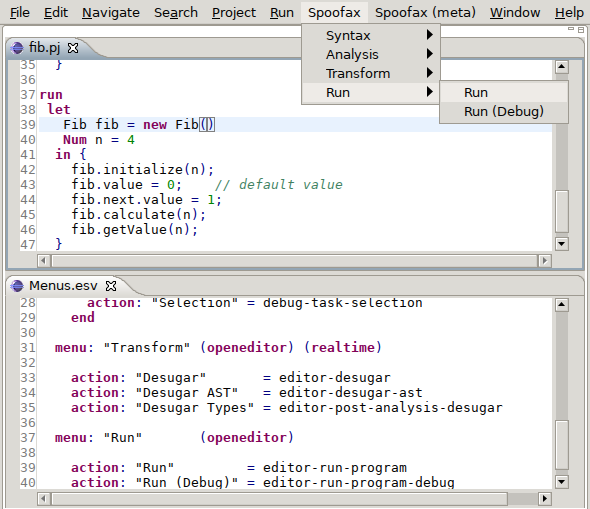
\includegraphics[width=0.6\textwidth]{./img/menu-actions.png}
\caption{\label{fig:menu-actions}
A menu action for the paplj language defined using Spoofax. The bottom window shows the menu definition, the top window shows a program written in paplj.}
\end{figure}

Editor services are defined using a DSL called ESV, shown in the bottom
window of \cref{fig:menu-actions}. In the case of menus, their actions are
specified using Stratego. Since Stratego supports native strategies, these
actions can also be specified in Java. As such, Spoofax allows for defining
arbitrarily complex IDE actions.

Many of these editor services such as syntax highlighting and code
folding rules can be derived from the syntax
definition~\cite{Kats10c} and can be further customized if
needed. Taken together with the language definition, the editor
services provide a language with a complete and state-of-the-art IDE
experience~\cite{Kats10a}.
%%% Local Variables:
%%% mode: latex
%%% TeX-master: "../main"
%%% End:


\section{Read-Eval-Print Loops}
\label{sec:repl}

Many programming languages come with an interactive environment. This
interactive environment is an interface to the programming language's execution
engine. One common form of such an environment is an interface in which
expressions in a programming language are typed by the user, after which the
results of that expression are printed back to the user. Such an environment is
called a Read-Eval-Print Loop (REPL), although many different names are known,
including but not limited to \emph{language shell},
\emph{command-line interpreter} or \emph{interactive interpreter}. There
are subtle differences between these names and the name REPL. These are,
however, mostly of semantic value. In this report the term REPL is chosen,
because it conveys the notion of such an interactive environment well.

\subsection{Origin of REPLs}
\label{ssec:repl-origin}

The Lisp programming language is one of the first programming languages offering
such an interactive environment~\cite{Noyes92}. The name REPL comes from the
Lisp functions that implement it:

\begin{enumerate}
  \item The \texttt{read} function takes a user's input, which often is just one
    or several expressions as opposed to a complete compilation unit. It then
    parses this input and creates an AST.
  \item The AST created in the previous step is then passed on to the
    \texttt{eval} function, which evaluates it.
  \item The result yielded by the previous function is then printed out to the
    user by the \texttt{print} function.
  \item After having printed the result, the environment needs to \texttt{loop}
    back to the read state.
\end{enumerate}

Assuming the individual functions listed previously exist, a REPL can be created
in a single line of code simply by combining the functions:

\begin{lstlisting}[language=lisp]
(loop (print (eval (read))))
\end{lstlisting}

Lisp has a property called ``homoiconicity'': Lisp's syntax is similar to
its internal representation, resulting in the ability to infer a program's or
data object's state simply by reading its textual representation. Syntax and AST
are thus isomorphic, allowing data and code to be accessed and transformed
interchangeably.

In Lisp REPLs, therefore, arbitrary data objects yielded from a previous
expression can be used directly as input to the next expression. In programming
languages that do not belong to the Lisp family, homoiconicity is an unusual
feature. Interactive environments for these languages therefore often require
additional steps to read and evaluate expressions. This is part of the semantic
differences between the different names as mentioned in the introduction

\subsection{Advantages of REPLs}
\label{ssec:repl-advantages}

REPLs provide the ability to program interactively. Programming interactively
has multiple advantages.

When creating software solutions for an as of yet not well understood domain, it
is often not clear which data structures and algorithms are required. In such
cases, interactively developing and debugging software is an advantage over the
(oftentimes much slower) edit-compile-run-debug development style. This kind of
programming is called exploratory programming~\cite{Fritzson86}. Related to this
kind of exploration, programming interactively also provides a means for rapid
prototyping and bottom up programming~\cite{Graham93}.

The explorative and interactive features of a REPL also make it an excellent
tool for programmers to learn a new programming language. REPLs are also
combined with what is called literate programming to offer notebooks or language
playgrounds, as discussed in \cref{sec:literate-programming}.

\subsection{Execution Model}
\label{ssec:execution-model}

Every programming language defines an execution model, which specifies how
programs written in that language are executed. Among others, it specifies what
an indivisible unit of work is (a \emph{compilation unit}) and in what order
these units are executed. The implementation of an execution model is a compiler
and/or an interpreter. The execution model of a REPL shown in
\cref{fig:execution-model-repl} has a couple of differences with respect to that
of an interpreter or compiler.

One difference is what is considered an indivisible unit of work: a REPL might
accept singular expressions that a regular interpreter or compiler might
not. Usually the program is executed as a whole, without the need for smaller
blocks of execution. In contrast, when using a REPL, it might be desirable to be
able to execute say only a single statement as one unit of execution. The AST
output of the parsing step, as shown in \cref{fig:execution-model-repl}, can
therefore be a smaller unit than an AST found in the ordinary execution model.

Another difference between a compiler or an interpreter and a REPL is that a
REPL needs to dynamically maintain an environment such that each new expression
can be analyzed and evaluated within the environment of previously executed
expressions. For every expression entered, it thus needs to apply the outlined
steps again and update the environment it maintains in memory with the new
results. This could result in a different order of evaluation than when say an
interpreter executes a program as a whole.

\begin{figure}[t]
  \centering
  \includegraphics[width=\textwidth]{execution-model-repl}
  \caption{The execution model as shown in \cref{fig:spoofax-relations}, adapted
    for a REPL. The analysis and evaluation is done within the incrementally
    built environment of previously executed expressions.}
  \label{fig:execution-model-repl}
\end{figure}

\subsection{Functionality}
\label{ssec:repl-functionality}

Every REPL provided with a programming language has its own set of
functionality. However, a core set of functionalities, shared between all REPL
implementations, can be identified. To reach this core set of features,
well-known REPLs have been investigated and their features have been compiled
into a matrix as seen in \cref{table:feature-matrix}. These features are shortly
discussed below.

\begin{table}[]
\centering
\begin{tabular}{lccccccccc}
                                  & \rot{Python} & \rot{R} & \rot{\shortstack[c]{Common\\Lisp}} & \rot{\shortstack[c]{Haskell\\(GHCi)}} & \rot{Swift} \\
\toprule
Executes single expressions       & \cmark       & \cmark  & \cmark                             & \cmark                                & \cmark      \\
Executes statements               & \cmark       & \cmark  & \cmark                             & \cmark                                & \cmark      \\
Input history                     & \cmark       & \cmark  & \cmark                             & \cmark                                & \cmark      \\
Automatic binding of previously yielded values & \xmark & \xmark & N/A                          & \xmark                                & \cmark      \\
Persistent input history          & \cmark       & \cmark  & \xmark                             & \cmark                                & \cmark      \\
Multiline input editing           & \cmark       & \cmark  & \cmark                             & \cmark                                & \cmark      \\
Redefining identifiers            & \cmark       & \cmark  & N/A                                & \cmark                                & \cmark      \\
Error reporting                   & \cmark       & \cmark  & \cmark                             & \cmark                                & \cmark      \\
Semantic code completion          & \cmark       & \xmark  & N/A                                & \xmark                                & \cmark      \\
Help or documentation system      & \cmark       & \cmark  & \cmark                             & \xmark                                & \xmark      \\
Additional commands to the REPL   & \xmark       & \xmark  & \cmark                             & \cmark                                & \cmark      \\
Nested REPLs to enable debugging  & \xmark       & \xmark  & \cmark                             & \xmark                                & \xmark      \\
\bottomrule
\end{tabular}
\caption{A feature comparison of several well-known REPLs}
\label{table:feature-matrix}
\end{table}

\paragraph{Input history} REPLs keep a history of inputs, such that previously
entered expressions can be retrieved.

\paragraph{Automatic binding of previously yielded values} When an expression
has been evaluated, the yielded result is bound to an automatically created
identifier, such that it can be reused easily in future expressions.

\paragraph{Persistent history} The input history as discussed previously can be
recorded into a file (either per-project or globally) to enable a persistent
history of input.

\paragraph{Multiline input editing} Some constructs in a programming language
naturally span multiple lines. REPLs therefore provide multiline input editors
that recognise incomplete code and promptly switch to a multiline environment
when required.

\paragraph{Redefining identifiers} When using a REPL in an exploratory manner,
it is not uncommon to want to redefine an identifier's type or to completely
reimplement a method. In this way, a REPL can be different than its host
language, especially if the host language is a functional language that does not
allow variables' values to change once initiated.

\paragraph{Error reporting} A REPL typically has the same error reporting
functionality as an interpreter or a compiler, meaning it prints the error
message accompanied by the corresponding section of the source code.

\paragraph{Semantic code completion} Semantic code completion is a helpful tool
to provide an overview of the often many APIs a developer works with, adding to
the explorative nature of a REPL. Note that this is a restriction of syntactic
completion, which is offered by all the studied REPLs.

\paragraph{Help or documentation system} The exploratory nature of a REPL means
that one will often see new methods. Some REPLs (most notably Python's REPL with
Python's docstrings) offer a documentation system, so that the developer does
not have to exit the REPL to look up documentation.

\paragraph{Additional commands to the REPL} Some REPLs offer additional commands
to inspect the environment or to control their behavior. These commands are
oftentimes not in the syntax of the host language and are highly diverse between
REPL implementations. A notable example of a REPL offering such commands is
Haskell's GHCi~\cite{GHCi-commands}.

\paragraph{Nested REPLs to enable debugging} A notable feature of (mostly) Lisp
REPLs is that in case of an error, a new REPL is spawned inside the context of
this error. This REPL then has additional commands (see the previous feature) to
enable debugging and inspection of the error state. When the user has
resolved the error, the nested REPL exits and the user is returned to the
parent REPL. This can go to arbitrary depths.

%%% Local Variables:
%%% mode: latex
%%% TeX-master: "../main"
%%% End:


%%% Local Variables:
%%% mode: latex
%%% TeX-master: "main"
%%% End:
